% Options for packages loaded elsewhere
% Options for packages loaded elsewhere
\PassOptionsToPackage{unicode}{hyperref}
\PassOptionsToPackage{hyphens}{url}
\PassOptionsToPackage{dvipsnames,svgnames,x11names}{xcolor}
%
\documentclass[
  british,
  a4paper,
]{article}
\usepackage{xcolor}
\usepackage{amsmath,amssymb}
\setcounter{secnumdepth}{-\maxdimen} % remove section numbering
\usepackage{iftex}
\ifPDFTeX
  \usepackage[T1]{fontenc}
  \usepackage[utf8]{inputenc}
  \usepackage{textcomp} % provide euro and other symbols
\else % if luatex or xetex
  \usepackage{unicode-math} % this also loads fontspec
  \defaultfontfeatures{Scale=MatchLowercase}
  \defaultfontfeatures[\rmfamily]{Ligatures=TeX,Scale=1}
\fi
\usepackage{lmodern}
\ifPDFTeX\else
  % xetex/luatex font selection
\fi
% Use upquote if available, for straight quotes in verbatim environments
\IfFileExists{upquote.sty}{\usepackage{upquote}}{}
\IfFileExists{microtype.sty}{% use microtype if available
  \usepackage[]{microtype}
  \UseMicrotypeSet[protrusion]{basicmath} % disable protrusion for tt fonts
}{}
\makeatletter
\@ifundefined{KOMAClassName}{% if non-KOMA class
  \IfFileExists{parskip.sty}{%
    \usepackage{parskip}
  }{% else
    \setlength{\parindent}{0pt}
    \setlength{\parskip}{6pt plus 2pt minus 1pt}}
}{% if KOMA class
  \KOMAoptions{parskip=half}}
\makeatother
% Make \paragraph and \subparagraph free-standing
\makeatletter
\ifx\paragraph\undefined\else
  \let\oldparagraph\paragraph
  \renewcommand{\paragraph}{
    \@ifstar
      \xxxParagraphStar
      \xxxParagraphNoStar
  }
  \newcommand{\xxxParagraphStar}[1]{\oldparagraph*{#1}\mbox{}}
  \newcommand{\xxxParagraphNoStar}[1]{\oldparagraph{#1}\mbox{}}
\fi
\ifx\subparagraph\undefined\else
  \let\oldsubparagraph\subparagraph
  \renewcommand{\subparagraph}{
    \@ifstar
      \xxxSubParagraphStar
      \xxxSubParagraphNoStar
  }
  \newcommand{\xxxSubParagraphStar}[1]{\oldsubparagraph*{#1}\mbox{}}
  \newcommand{\xxxSubParagraphNoStar}[1]{\oldsubparagraph{#1}\mbox{}}
\fi
\makeatother


\usepackage{longtable,booktabs,array}
\newcounter{none} % for unnumbered tables
\usepackage{calc} % for calculating minipage widths
% Correct order of tables after \paragraph or \subparagraph
\usepackage{etoolbox}
\makeatletter
\patchcmd\longtable{\par}{\if@noskipsec\mbox{}\fi\par}{}{}
\makeatother
% Allow footnotes in longtable head/foot
\IfFileExists{footnotehyper.sty}{\usepackage{footnotehyper}}{\usepackage{footnote}}
\makesavenoteenv{longtable}
\usepackage{graphicx}
\makeatletter
\newsavebox\pandoc@box
\newcommand*\pandocbounded[1]{% scales image to fit in text height/width
  \sbox\pandoc@box{#1}%
  \Gscale@div\@tempa{\textheight}{\dimexpr\ht\pandoc@box+\dp\pandoc@box\relax}%
  \Gscale@div\@tempb{\linewidth}{\wd\pandoc@box}%
  \ifdim\@tempb\p@<\@tempa\p@\let\@tempa\@tempb\fi% select the smaller of both
  \ifdim\@tempa\p@<\p@\scalebox{\@tempa}{\usebox\pandoc@box}%
  \else\usebox{\pandoc@box}%
  \fi%
}
% Set default figure placement to htbp
\def\fps@figure{htbp}
\makeatother



\ifLuaTeX
\usepackage[bidi=basic,shorthands=off]{babel}
\else
\usepackage[bidi=default,shorthands=off]{babel}
\fi
\ifLuaTeX
  \usepackage{selnolig} % disable illegal ligatures
\fi


\setlength{\emergencystretch}{3em} % prevent overfull lines

\providecommand{\tightlist}{%
  \setlength{\itemsep}{0pt}\setlength{\parskip}{0pt}}



 


\makeatletter
\@ifpackageloaded{tcolorbox}{}{\usepackage[skins,breakable]{tcolorbox}}
\@ifpackageloaded{fontawesome5}{}{\usepackage{fontawesome5}}
\definecolor{quarto-callout-color}{HTML}{909090}
\definecolor{quarto-callout-note-color}{HTML}{0758E5}
\definecolor{quarto-callout-important-color}{HTML}{CC1914}
\definecolor{quarto-callout-warning-color}{HTML}{EB9113}
\definecolor{quarto-callout-tip-color}{HTML}{00A047}
\definecolor{quarto-callout-caution-color}{HTML}{FC5300}
\definecolor{quarto-callout-color-frame}{HTML}{acacac}
\definecolor{quarto-callout-note-color-frame}{HTML}{4582ec}
\definecolor{quarto-callout-important-color-frame}{HTML}{d9534f}
\definecolor{quarto-callout-warning-color-frame}{HTML}{f0ad4e}
\definecolor{quarto-callout-tip-color-frame}{HTML}{02b875}
\definecolor{quarto-callout-caution-color-frame}{HTML}{fd7e14}
\makeatother
\makeatletter
\@ifpackageloaded{caption}{}{\usepackage{caption}}
\AtBeginDocument{%
\ifdefined\contentsname
  \renewcommand*\contentsname{Table of contents}
\else
  \newcommand\contentsname{Table of contents}
\fi
\ifdefined\listfigurename
  \renewcommand*\listfigurename{List of Figures}
\else
  \newcommand\listfigurename{List of Figures}
\fi
\ifdefined\listtablename
  \renewcommand*\listtablename{List of Tables}
\else
  \newcommand\listtablename{List of Tables}
\fi
\ifdefined\figurename
  \renewcommand*\figurename{Figure}
\else
  \newcommand\figurename{Figure}
\fi
\ifdefined\tablename
  \renewcommand*\tablename{Table}
\else
  \newcommand\tablename{Table}
\fi
}
\@ifpackageloaded{float}{}{\usepackage{float}}
\floatstyle{ruled}
\@ifundefined{c@chapter}{\newfloat{codelisting}{h}{lop}}{\newfloat{codelisting}{h}{lop}[chapter]}
\floatname{codelisting}{Listing}
\newcommand*\listoflistings{\listof{codelisting}{List of Listings}}
\makeatother
\makeatletter
\makeatother
\makeatletter
\@ifpackageloaded{caption}{}{\usepackage{caption}}
\@ifpackageloaded{subcaption}{}{\usepackage{subcaption}}
\makeatother
\usepackage{bookmark}
\IfFileExists{xurl.sty}{\usepackage{xurl}}{} % add URL line breaks if available
\urlstyle{same}
% fallback for those not using the hyperref driver hyperxmp:
\makeatletter
\@ifundefined{xmpquote}{\newcommand{\xmpquote}[1]{#1}}{}
\makeatother
\hypersetup{
  pdftitle={A trading signal that did not survive honest testing},
  pdfauthor={Carlos Galindo},
  pdflang={en-GB},
  colorlinks=true,
  linkcolor={blue},
  filecolor={Maroon},
  citecolor={Blue},
  urlcolor={Blue},
  pdfcreator={LaTeX via pandoc}}


\title{A trading signal that did not survive honest testing}
\usepackage{etoolbox}
\makeatletter
\providecommand{\subtitle}[1]{% add subtitle to \maketitle
  \apptocmd{\@title}{\par {\large #1 \par}}{}{}
}
\makeatother
\subtitle{A pre-registered, net-of-cost, out-of-sample test of a
time-varying-sensitivity trading rule found no edge, and the null was
reported as such}
\author{Carlos Galindo}
\date{}
\begin{document}
\maketitle


\begin{tcolorbox}[enhanced jigsaw, arc=.35mm, bottomrule=.15mm, breakable, colback=white, colframe=quarto-callout-note-color-frame, left=2mm, leftrule=.75mm, opacityback=0, rightrule=.15mm, toprule=.15mm]

\vspace{-3mm}\textbf{At a glance}\vspace{3mm}

\begin{itemize}
\tightlist
\item
  \textbf{Question.} Does a model in which a precious metal's daily
  sensitivity to real yields and the dollar drifts over time give a
  tradable, real-time, out-of-sample edge after costs?
\item
  \textbf{Approach.} A design fixed in writing before any result was
  produced: four benchmarks, two cost levels, a stated number of
  configurations tried, and a mechanical verdict rule.
\item
  \textbf{Finding.} No edge. The signal lost money net of costs, trailed
  buy-and-hold, and its deflated Sharpe ratio was essentially zero. A
  second, simpler calendar rule on equities also failed the same bar.
\item
  \textbf{Why it matters.} Statistical forecast skill is not an economic
  edge, and a test that can say ``no'' in advance is worth more than a
  backtest that always finds something.
\end{itemize}

\end{tcolorbox}

\subsection{The question}\label{the-question}

A precious metal's relationship with real interest rates and the dollar
is one of the best-known regularities in macro-finance. Higher real
yields raise the opportunity cost of holding a non-yielding asset, and a
stronger dollar makes the metal dearer for everyone else. The
relationship is not stable, though: it weakened markedly in recent
years, which is the usual motivation for letting the sensitivities vary
over time.

That motivation invites a trading idea. If the sensitivities can be
tracked in real time, then today's moves in yields and the dollar should
predict tomorrow's move in the metal, and a rule that goes long or short
accordingly should make money. The question here is whether that is
true, and the way the question is asked matters as much as the answer.
Trading-rule research is a standard setting for self-deception. With
enough variants, enough sample splits and enough tolerance for
look-ahead, almost any rule can be made to look profitable. The aim was
to remove those degrees of freedom before looking at any result.

\subsection{Approach}\label{approach}

\textbf{Model.} Daily returns on the metal were regressed on daily
changes in a long-term real interest rate and in the trade-weighted
dollar, with both coefficients following random walks. The coefficients
are estimated by a state-space filter that uses only information up to
each date, never a smoothed estimate that sees the future. The rule is
direct: the day's fitted driver contribution gives a sign, and the
position next day is long or short one unit according to that sign. In
other words, it bets that the contemporaneous relationship persists one
day forward.

\textbf{Data.} Daily closes of an exchange-traded fund tracking a
precious metal, a long-term real interest rate and a broad
trade-weighted dollar measure, 5,404 aligned trading days from late 2004
to mid-2026. These are market and official closes, so there is no
revision problem. Two substitutions of series, forced by access limits,
were logged in the design and both were judged to be conservative.

\textbf{Walk-forward discipline.} The two variance parameters of the
filter were fitted by predictive likelihood on an expanding window of
past data only and re-estimated once a year. A two-year warm-up preceded
trading, which left 4,898 out-of-sample trading days from late 2006 to
mid-2026. Nothing was tuned to the known 2022 to 2025 breakdown in the
metal--yield relationship, and a regime-switching variant that would
have been designed to fit it was explicitly excluded.

\textbf{Benchmarks that must all be beaten.} Buy-and-hold on the metal;
the same signal with coefficients from a 60-day rolling regression,
which isolates whether the filter adds anything; a rule that simply goes
long when real yields fall; and a momentum rule.

\textbf{Costs.} Two basis points per unit of turnover, with five basis
points as a robustness case.

\textbf{Multiple testing and the decision rule.} Performance was judged
on the annualised Sharpe ratio and on the deflated Sharpe ratio, which
corrects for the number of configurations tried, for skewness and fat
tails, and for sample length. Six configurations were counted honestly.
The verdict was fixed in advance with three possible outcomes: edge
confirmed only if the signal beat both buy-and-hold and the rolling
regression and its deflated Sharpe ratio exceeded 0.95; ambiguous if it
beat them on raw Sharpe only; no edge otherwise. The prior, recorded in
advance, was that the null was the expected outcome, because the
metal--yield link is largely a low-frequency, contemporaneous
phenomenon.

\subsection{What the work shows}\label{what-the-work-shows}

The verdict was \textbf{no edge; the null holds}. The table sets out the
net-of-cost results over the 4,898-day window.

{\def\LTcaptype{none} % do not increment counter
\begin{longtable}[]{@{}llll@{}}
\toprule\noalign{}
Strategy & Sharpe (annual) & Deflated Sharpe & Annual return \\
\midrule\noalign{}
\endhead
\bottomrule\noalign{}
\endlastfoot
Time-varying signal, 2 bp & -0.165 & 0.002 & -3.0\% \\
Time-varying signal, 5 bp & -0.579 & 0.000 & -10.5\% \\
Rolling-regression signal, 2 bp & -0.353 & 0.000 & -6.4\% \\
Sign of real-yield change, 2 bp & -0.280 & 0.000 & -4.9\% \\
Metal momentum, 2 bp & -0.510 & 0.000 & -9.3\% \\
Buy and hold, metal & 0.482 & 0.475 & 8.8\% \\
\end{longtable}
}

Three results stand out. First, every active rule lost money after
costs, and the main signal lost money even at the lowest cost level; at
five basis points the annual loss was 10.5\%. Second, the benchmark that
mattered most, simply holding the metal, earned a Sharpe ratio of 0.482
against -0.165 for the signal. Third, the deflated Sharpe ratio of the
signal was 0.002 against a requirement of 0.95. With six configurations
the deflated hurdle for the annualised Sharpe ratio was 0.496, which
even buy-and-hold did not clear on the deflated measure (0.475).

The filter did do something useful relative to the naive version: it
beat the rolling regression on Sharpe (-0.165 against -0.353). A test of
equal predictive accuracy on one-day-ahead squared errors also favoured
the filter decisively. The filter shrinks its coefficients towards zero
and so forecasts with less noise. Yet it still lost money. That is the
central lesson, and it is easy to state in a sentence: \emph{statistical
forecast skill is not an economic edge.} A model can have lower squared
error and still fail to profit, because the positions that matter are
the extreme calls, and the cost and sign of those calls are not what
mean squared error measures.

\begin{figure}

\centering{

\pandocbounded{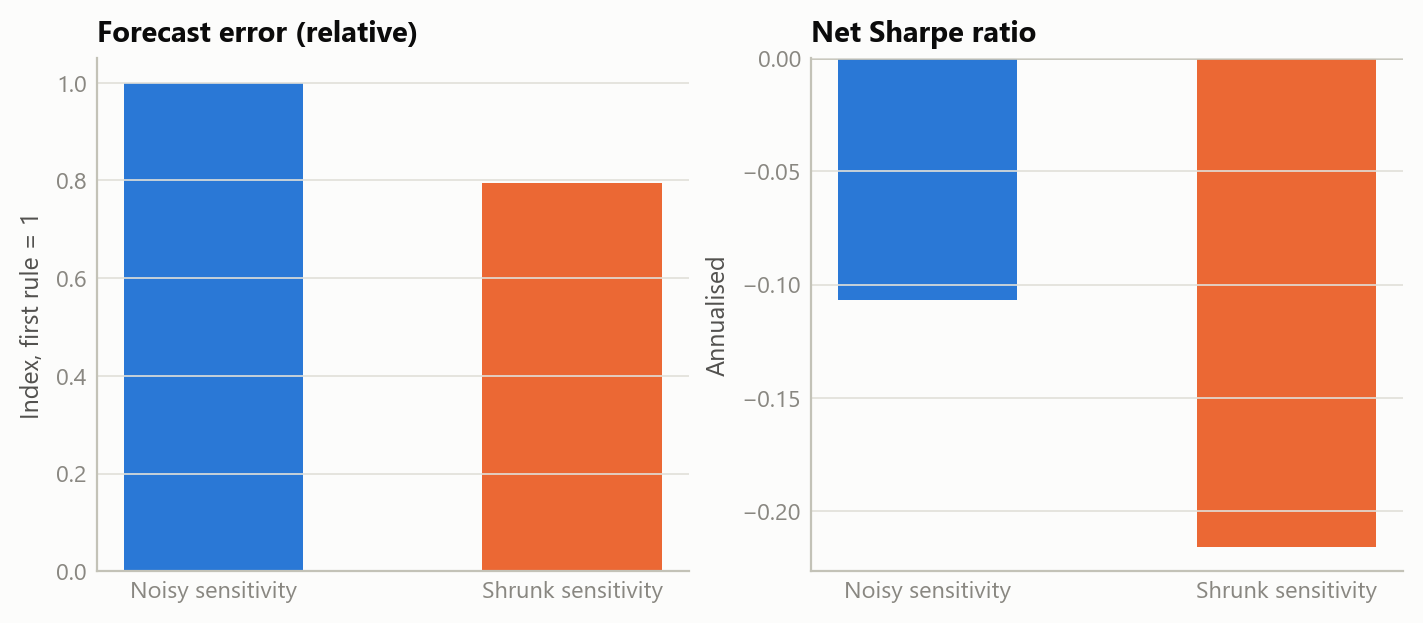
\includegraphics[keepaspectratio]{index_files/figure-latex/fig-forecast-vs-profit-output-1.png}}

}

\caption{\label{fig-forecast-vs-profit}Lower forecast error without a
profit: relative forecast error and net Sharpe for two rules with no
true edge (simulated data).}

\end{figure}%

The next figure shows why the deflation matters. Among many rules with
no true edge, the best one will look impressive, and the more are tried
the better the best looks.

\begin{figure}

\centering{

\pandocbounded{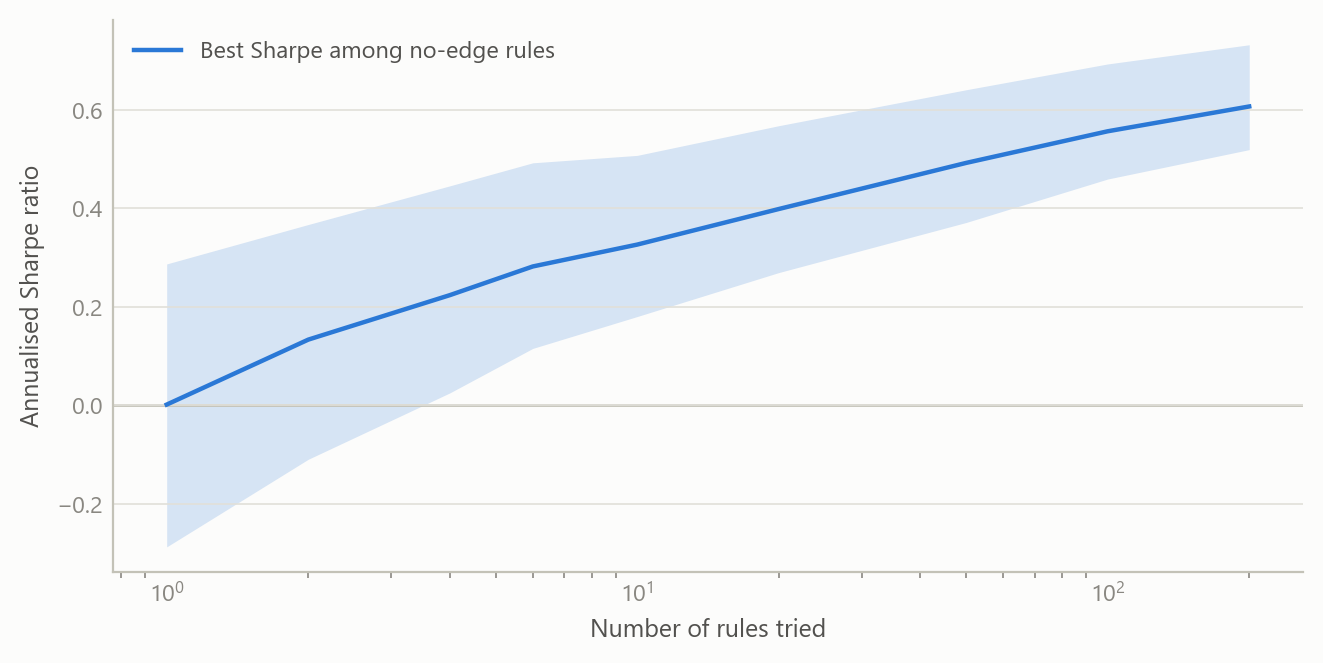
\includegraphics[keepaspectratio]{index_files/figure-latex/fig-deflation-output-1.png}}

}

\caption{\label{fig-deflation}The best of many no-edge rules looks good;
the hurdle rises with the number tried (simulated data).}

\end{figure}%

\begin{figure}

\centering{

\pandocbounded{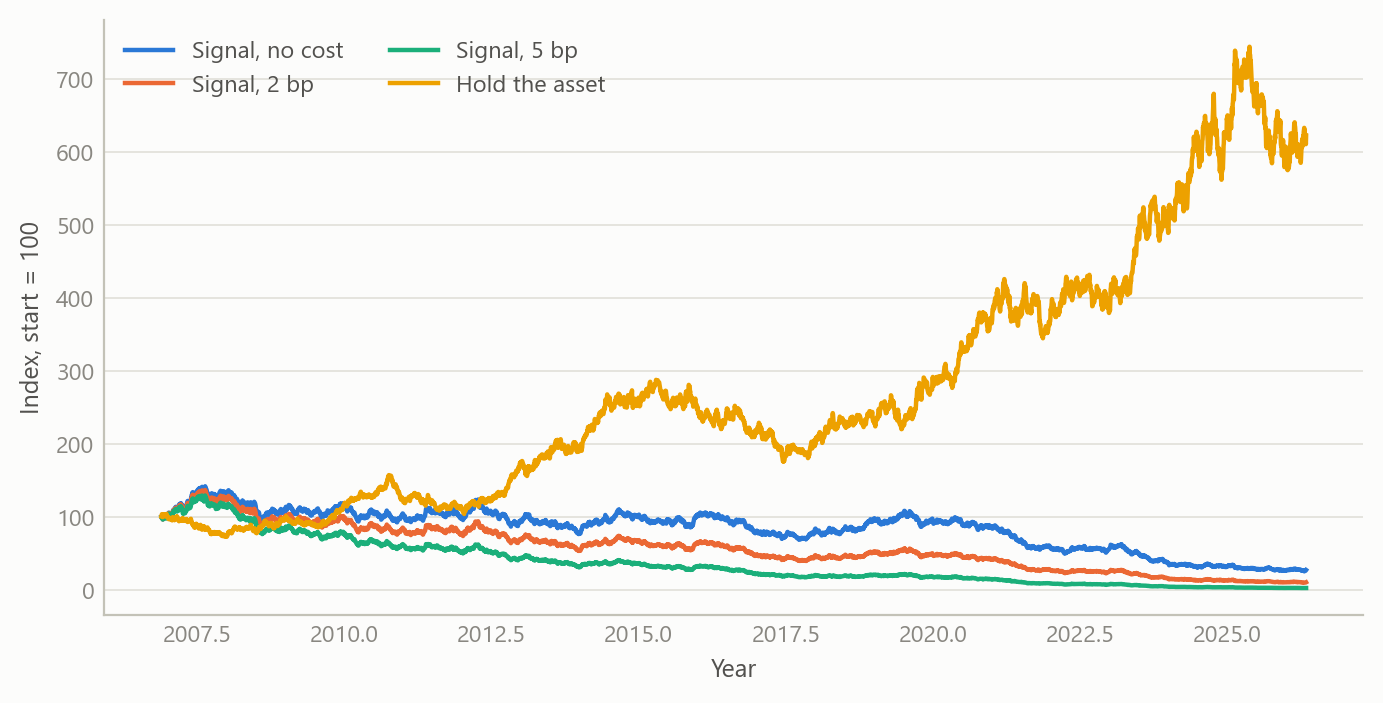
\includegraphics[keepaspectratio]{index_files/figure-latex/fig-cumulative-output-1.png}}

}

\caption{\label{fig-cumulative}Cumulative net return of a no-edge signal
at three cost levels, against holding the asset (simulated data).}

\end{figure}%

The same discipline was applied to a second candidate chosen as a simple
contrast: a fixed calendar rule that holds equities only around the turn
of the month. A fixed calendar rule has no fitted parameters, so it is
walk-forward clean by construction. Over 8,166 trading days it earned a
Sharpe ratio of 0.376 against 0.548 for buy-and-hold, with a deflated
Sharpe ratio of 0.927, short of the 0.95 bar. It was in the market 24\%
of the time and captured about 8\% of the cumulative log return.
Verdict: no edge, reported the same way.

\subsection{Insights}\label{insights}

\begin{enumerate}
\def\labelenumi{\arabic{enumi}.}
\tightlist
\item
  \textbf{Fix the verdict before the result.} The decisive feature was a
  mechanical rule written first, with the prior stated, so a null could
  not be reinterpreted as a near miss.
\item
  \textbf{A simple benchmark is the real opponent.} Beating a naive
  version of the same model was not enough; buy-and-hold and two crude
  rules were the bar, and the sophisticated model lost to all of them on
  a net basis.
\item
  \textbf{Count the trials.} Six configurations lifted the deflated
  hurdle to 0.496 in annual Sharpe terms. Without the correction, a
  modest positive Sharpe ratio would have looked like a finding.
\item
  \textbf{Contemporaneous is not predictive.} The relationship that
  motivates the model is real and strong at the same date, and it does
  not carry one day forward in a way that survives costs.
\item
  \textbf{A clean null is an output.} The design was built so that a
  null would be a successful, useful result, and it is reported straight
  with a no-go decision and no capital deployed.
\end{enumerate}

\subsection{Limits and next steps}\label{limits-and-next-steps}

The test covers one family of rules on one asset at daily frequency. It
says nothing about intraday strategies, options, leverage or volatility
targeting, other instruments, or regime-switching variants, all of which
were declared out of scope in advance and none of which can rescue this
result. The data substitutions were logged, though a different dollar
measure or real-yield definition could shift the numbers slightly. Costs
are retail-scale and applied as a flat charge per unit of turnover, with
no market impact. The sample is long, but a single path of history is
still one draw.

Natural extensions would be to apply the same pre-registered template to
other candidate signals, so that the number of trials is tracked across
a whole research programme and not only within one test, and to examine
low-frequency levels relationships, where the original motivation lives,
with the same standards.

\subsection{About the evidence}\label{about-the-evidence}

The results in the text are from the project's own out-of-sample
backtest, completed in 2026 on daily market and official data, with no
capital deployed. The figures here are illustrative: they are simulated
to share the horizon, sample length and cost structure of the real test
and demonstrate the logic, not to reproduce its results.

Figures and tables marked \emph{simulated} are generated from simulated
data built to share the structure of the analysis (its variables,
horizons and frequencies). They show how the method works and what its
output looks like; they are not the project's results. Results stated in
the text are the project's own. Methods are described at the level of a
methods section. Code and data pipelines are not reproduced here.




\end{document}
